\begin{itemize}
    \item Módulo 1: ``O Problema da Cerca"
    
    ``Com 80 metros de cerca um fazendeiro deseja circundar uma região retangular junto a um rio para confinar alguns animais. O lado da região retangular junto a margem do rio não é cercado. Quanto deve ser x, a medida em metros da base da região retangular, para que a área cercada A seja a maior possível?”.
    
    É uma contextualização clássica de problema de otimização, que trabalha simultaneamente as noções de perímetro e área, evidenciando suas relações e diferenças com elementos muito comuns: cerca e área de terreno. Tem como pré-requisitos área e perímetro de retângulo, o Teorema de Pitágoras.
    
    
    \item Módulo 2: ``O Problema do Barbante: Quadrado e Círculo"
    
    ``Um fio de barbante de 10 metros de comprimento pode ser usado ou para construir um quadrado, ou para construir um círculo ou ele pode ser cortado em dois pedaços (não necessariamente de mesmo tamanho) de modo que um dos pedaços é usado para construir um quadrado e o outro pedaço é usado para construir um círculo. Quanto deve ser x, a medida em metros do pedaço do barbante usado para construir o quadrado, para que a soma S das áreas das figuras produzidas seja a maior possível? Quanto deve ser x, a medida em metros do pedaço do barbante usado para construir o quadrado, para que a soma S das áreas das figuras produzidas seja a menor possível?”.

    Trata da comparação entre a relação área-perímetro entre figuras geométricas diferentes --- círculo e quadrado, no caso. Tem como pré-requisitos área e perímetro de quadrados, área e perímetro de círculos, o Teorema de Pitágoras. 
    
    \item Módulo 3: ``O Problema do Barbante: Quadrado e Triângulo"
    
    % \begin{citacao}
    ``Um fio de barbante de 10 metros de comprimento pode ser usado ou para construir um quadrado, ou para construir um triângulo equilátero ou ele pode ser cortado em dois pedaços (não necessariamente de mesmo tamanho) de modo que um dos pedaços é usado para construir um quadrado e o outro pedaço é usado para construir um triângulo equilátero. Quanto deve ser x, a medida em metros do pedaço do barbante usado para construir o quadrado, para que a soma S das áreas das figuras produzidas seja a maior possível? Quanto deve ser x, a medida em metros do pedaço do barbante usado para construir o quadrado, para que a soma S das áreas das figuras produzidas seja a menor possível?”
    % \cite{cdme-pot}
    % \end{citacao}
    
    Módulo análogo ao anterior, agora com as figuras quadrado e triângulo equilátero. Serve como complemento e reforço para que o aluno entenda de onde vêm as proporções que maximizam a soma da área das figuras. Trata da comparação entre a relação área-perímetro entre figuras geométricas diferentes --- círculo e quadrado, no caso. Tem como pré-requisitos área e perímetro de quadrados, área e perímetro de triângulos equiláteros, o Teorema de Pitágoras. 
    
    \item Módulo 4: ``O Problema da Janela Normanda"
    
    ``Uma janela normanda tem o formato da justaposição de um semicírculo sobre um retângulo. Considerando as janelas normandas com perímetro igual a 9 m, quanto deve ser x, a medida em metros da base do retângulo que compõe a janela, para que a área A da janela seja a maior possível?”
    
    Aborda a relação que se apresenta entre o perímetro e a área de uma figura geométrica. Tem como pré-requisitos perímetro e área de retângulos, perímetro e área de semicírculos.
    
    \item Módulo 5: ``O Problema do Triângulo Isósceles"
    
    ``Considerando os triângulos isósceles com dois lados de medidas iguais a 3 m, quanto deve ser x, a medida em metros da base triângulo isósceles, para que a área A do triângulo seja a maior possível?”.
    
    Esse módulo traz a relação implícita entre ângulo e base de um triângulo com dois lados fixos, podendo ser usada para instigar o pensamento trigonométrico. tem como pré-requisitos área e perímetro de triângulos, o Teorema de Pitágoras.
    
    \item Módulo 6: ``Um Problema Geométrico"
    
     ``Considere pontos A, B, C, H e M no plano. O ponto H pertence ao segmento de extremidades B e C, de modo que a distância entre B e H é igual a 2 m e a distância entre H e C é igual a 3 m. O segmento AH é perpendicular ao segmento BC e ele tem medida igual a 5 m. O ponto M pertence ao segmento de extremidades A e H. Quanto deve ser x, a medida em metros da distância entre os pontos A e M, para que o comprimento total L de fios ligando M aos pontos A, B e C seja o menor possível?”
     
     É o primeiro módulo a não citar área, focando no teorema de Pitágoras e na relação cartesiana da distância entre um ponto fixo e um outro que varia em um eixo. Tem como pré-requisitos distância entre pontos no plano, o Teorema de Pitágoras.
    
    \item Módulo 7: ``O Problema do Caminho para A Horta"
    
    ``Um agricultor está em sua casa C situada a 80 metros da margem retilínea de um rio. Ele quer encher primeiro o seu regador de água em um ponto M na margem deste rio e, depois, se dirigir para sua horta H, situada a 50 metros da margem do rio. A distância entre os pés A e B das perpendiculares traçadas de C e H sobre a margem do rio é igual a 100 metros. Considere um sistema de coordenadas onde A = (0, 0), B = (100, 0), C = (0, 80), H = (100, 50) e M = (x, 0). Quanto deve ser x, a abscissa do ponto M sobre o eixo x, para que o comprimento d do trajeto casa (C), rio (M) e horta (H) seja o menor possível?”
    
    Pela primeira vez, o enunciando traz explicitamente a notação utilizada em planos cartesianos, e apresenta os primeiros conceitos relacionados à Geometria Analítica, instigando esse tipo de pensamento na cabeça do aluno sem necessariamente se aprofundar. O exercício do módulo em si é semelhante ao anterior, então valem os mesmos comentários, e os pré-requisitos são distância entre pontos no plano, o Teorema de Pitágoras.
    
    \item Módulo 8: ``O Problema da Distância entre Ponto e Reta"
    
    ``Dado um ponto A no plano cartesiano, quanto deve ser x para que a distância d entre A e M = (x, -2x + 4) (um ponto da reta y = -2x + 4) seja a menor possível?”
    
    O módulo traz, inserindo o conceito de função dentro do exercício de função, uma situação inteiramente composta de objetos Matemáticos. Dá, assim, oportunidade para o aluno desenvolver a sua capacidade de abstração, com o auxílio do gráfico. Tem como pré-requisito distância entre pontos no plano.
    
    \item Módulo 9: ``O Problema da Distância entre Ponto e Parábola"

    ``Dado um ponto A no plano cartesiano, quanto deve ser x para que a distância d entre A e M = (x, x$^2$) (um ponto da parábola y = x$^2$) seja a menor possível?”
    
    Assim como no módulo anterior, este propõe uma atividade contextualizada apenas com abstrações Matemáticas. Ao trabalhar com um objeto pouco frequente em problemas que envolvem distâncias, traz um questionamento mais aprofundado sobre a definição de distância de um ponto a um conjunto, no caso a parábola. Busca-se na atividade o ponto da parábola cuja distância ao ponto dado é mínima, isto é, o ponto que realiza a distância entre parábola e ponto.
    
    % caracterizar a distância de um ponto a um objeto, uma determinada curva a menor distância, ponto que pode ser resolvido intuitivamente e sem mais reflexões no módulo anterior. Tem como pré-requisito distância entre pontos no plano.
    
    \item Módulo 10: ``O Problema do Retângulo: Área e Perímetro"
    
    ``Considerando os retângulos de área igual a 3 m$^2$, quanto deve ser x, a medida em metros da base do retângulo, para que o perímetro y do retângulo seja o menor possível?”
    
    Aqui o projeto aborda novamente a relação de área e perímetro, dessa vez invertendo a relação proposta anteriormente, avaliando o perímetro em função da área. Tem como pré-requisitos área e perímetro de retângulo.
    
    \item Módulo 11: ``O Problema do Retângulo Inscrito num Círculo"
    
    ``Queremos encaixar (inscrever) dentro de um círculo um retângulo com a maior área possível. Se o círculo tem 3 metros de raio, quanto deve ser x, a medida em metros da base do retângulo, para que a área A do retângulo seja a maior possível?”
    
    Voltando a tratar o conceito de área em Geometria Plana, o módulo trabalha a ideia do problema de otimização com restrição com esse problema simples, oferecendo uma representação gráfica do problema. Tem como pré-requisitos área e perímetro de retângulos, o Teorema de Pitágoras.

    \item Módulo 12: ``O Problema do Triângulo Inscrito num Círculo"
    
    ``Queremos encaixar (inscrever) dentro de um círculo um triângulo isósceles com a maior área possível. Se o círculo tem 3 metros de raio, quanto deve ser x, a medida em metros da altura do triângulo, para que a área A do triângulo seja a maior possível?”
    
    Similarmente ao módulo anterior, explora a variação da área de um triângulo isósceles, com a restrição de estar inscrito em um círculo de raio fixo. Traz um exercício muito interessante envolvendo o teorema de Pitágoras, e tem com pré-requisitos área de triângulos, e o já mencionado Teorema de Pitágoras.
    
    \item Módulo 13: ``O Problema da Bobina do Transformador"
    
    ``Na construção de um transformador de corrente alternada, insere-se na bobina circular do transformador um núcleo de ferro cuja seção transversal tem o formato de uma cruz. É importante que esta seção transversal tenha a maior área possível. Se o raio da seção transversal circular da bobina mede 18 milímetros e se x representa a metade da medida, em milímetros, dos lados da cruz cujas extremidades estão sobre a seção circular, quanto deve ser x para que a área A da cruz seja a maior possível?"

    Esse módulo apresenta uma contextualização muito interessante vinda da engenharia, e começa a trabalhar com áreas não triviais. Nela o aluno deve quebrar a área da \textit{cruz} em áreas menores que ele consegue calcular, estimulando o pensamento de \textit{dividir para conquistar}, tão importante na matemática. Tem como pré-requisitos área de retângulos, o Teorema de Pitágoras.
    
    \item Módulo 14: ``O Problema da Caixa"
    
    ``Quadrados iguais são cortados dos cantos de uma folha de papelão retangular medindo 30 cm por 50 cm. As abas que sobram são então dobradas para cima de modo a formar uma caixa sem tampa. Quanto deve ser x, a medida em centímetros dos lados dos quadrados que são retirados da folha de papelão, para que o volume V da caixa seja o maior possível?”
    
    A partir desse módulo as atividades passam a tratar de geometria em três dimensões. O projeto inicia essa sequência com uma atividade que trata da relação entre área e volume em uma figura geométrica espacial. Tem como pré-requisitos área e perímetro de retângulos, volume de prismas retos quadrangulares.
    
    \item Módulo 15: ``O Problema da Caixa com Tampa"
    
    ``Um fabricante quer construir caixas com tampa a partir de uma folha de papelão retangular medindo 10 cm por 16 cm. Para construir a caixa, dois quadrados e dois retângulos são removidos dos cantos da folha de papelão. As abas que sobram são então dobradas para cima de modo a formar uma caixa com tampa. Quanto deve ser x, a medida em centímetros dos lados dos quadrados que são retirados da folha de papelão, para que o volume V da caixa seja o maior possível?”
    
    O módulo é muito similar ao anterior, com a diferença do formato da figura tratada. O fato de a caixa não ter tampa altera o corte feito, e assim muda a quantidade máxima de papelão que pode ser utilizada em uma situação dessa, excelente para promover o pensamento crítico. Tem como pré-requisitos área e perímetro de retângulos, volume de prismas retos quadrangulares.
    
    \item Módulo 16: ``O Problema do Bebedouro"
    
    ``Um bebedouro será construído na forma de um prisma reto cuja altura mede 7 m e cujas bases são trapézios. Cada trapézio tem base menor e laterais de medidas sempre iguais a 1 m. Se x representa a medida, em radianos, do ângulo entre uma lateral e uma altura de cada um dos dois trapézios congruentes usados na construção do bebedouro, quanto deve ser x para que a forma do bebedouro correspondente tenha o maior volume V possível?”
    
    Esse módulo se mostra interessante para abordar trigonometria, já que precisamos de uma maneira de relacionar os comprimentos das arestas com a variável sobre a qual temos algum controle: o ângulo. A questão do bebedouro se enchendo de água também traz a possibilidade de abordar o tema da semelhança entre sólidos. Tem como pré-requisitos área de triângulos, área de retângulos, trigonometria no triângulo retângulo, volume de prismas retos, o Teorema de Pitágoras.
    
    \item Módulo 17: ``O Problema da Embalagem Piramidal"
    
    ``Um fabricante quer construir uma embalagem no formato de uma pirâmide regular de base quadrada a partir de uma folha de papelão quadrada medindo 2 m por 2 m. Para construir a embalagem, triângulos isósceles são removidos das laterais da folha de papelão. As pontas que sobram são então dobradas para cima de modo a formar uma pirâmide regular de base quadrada. Quanto deve ser x, a metade da medida em metros da diagonal da base quadrada da pirâmide, para que o volume V da embalagem seja o maior possível?”
    
    Outro módulo que se estende sobre a relação entre área e volume de um sólido específico através da planificação, oferecendo uma estratégia interessante para a obtenção da planificação de uma pirâmide a partir de uma superfície quadrada. Tem como pré-requisitos elementos métricos do triângulo isósceles, elementos métricos do quadrado, volume de pirâmides regulares, o Teorema de Pitágoras.
    
    \item Módulo 18: ``O Problema do Cone"
    
    ``Um copo no formato cônico é feito com um disco circular de papel, de centro O, do qual foi retirado um setor circular AOM e os lados OA e OM foram unidos. Os lados OA e OM têm medida 7 cm. Quanto deve ser x, a medida em radianos do ângulo AOM, para que o volume V do copo seja o maior possível?”
    
    O último módulo explicitamente sobre relação entre área e volume, agora introduzindo um sólido não poliédrico, explora a relação da área lateral do cone como o seu volume. Tem como pré-requisitos perímetro de arcos de círculo, volume de cones circulares, o Teorema de Pitágoras.
    
    \item Módulo 19: ``O Problema do Cilindro Inscrito numa Esfera"
    
    ``Queremos encaixar (inscrever) dentro de uma esfera um cilindro circular reto com o maior volume possível. Se a esfera tem 3 metros de raio, quanto deve ser x, a medida em metros do raio da base do cilindro, para que o volume V do cilindro seja o maior possível?”
    
    Módulo análogo ao número 11, possibilita a discussão das simetrias de figuras geradas a partir de rotações de uma figura plana. Os pré-requisitos são volume de cilindros circulares, o Teorema de Pitágoras.
    
    \item Módulo 20: ``O Problema do Cone Inscrito numa Esfera"
    
    ``Queremos encaixar (inscrever) dentro de uma esfera um cone circular reto com o maior volume possível. Se a esfera tem 3 metros de raio, quanto deve ser x, a medida em metros da altura do cone, para que o volume V do cone seja o maior possível?”
    
    Um exercício parecido com o do Módulo 11, agora trabalhado em 3 dimensões. Possibilita essa discussão da Geometria Plana presente em seções de figuras tridimensionais. Tem como pré-requisitos volume de cones circulares, o Teorema de Pitágoras.
    
    \item Módulo 21: ``O Problema da Pirâmide Inscrita numa Esfera"
    
    ``Queremos encaixar (inscrever) dentro de uma esfera uma pirâmide regular de base quadrada com o maior volume possível. Se a esfera tem 3 metros de raio, quanto deve ser x, a medida em metros da altura da pirâmide, para que o volume V da pirâmide seja o maior possível?”
    
    O último módulo atualmente mistura a noção de poliedro --- a pirâmide inscrita --- com sólidos não poliédricos --- a esfera ---, que pode promover questionamentos interessantes se comparado com a atividade anterior. Quando pontos da pirâmide encostam na esfera, e como essa informação difere do caso do cone e o cilindro inscritos? Tem como pré-requisitos volume de pirâmides regulares, o Teorema de Pitágoras.
\end{itemize}

\begin{figure}
    \centering
    
    \begin{subfigure}{0.3\textwidth}
    \centering
    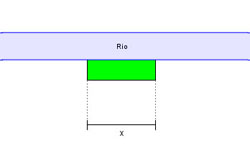
\includegraphics[width=.9\textwidth]{icones-modulos/pot-m-pce.jpg}
    \label{fig:pce-ic}
    \end{subfigure}
    \hfill
    \begin{subfigure}{0.3\textwidth}
    \centering
    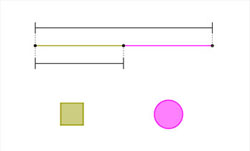
\includegraphics[width=.9\textwidth]{icones-modulos/pot-m-pbc.jpg}
    \label{fig:pbc-ic}
    \end{subfigure}
    \hfill
    \begin{subfigure}{0.3\textwidth}
    \centering
    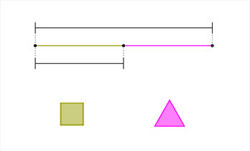
\includegraphics[width=.9\textwidth]{icones-modulos/pot-m-pbt.jpg}
    \label{fig:pbt-ic}
    \end{subfigure}
    
    \begin{subfigure}{0.3\textwidth}
    \centering
    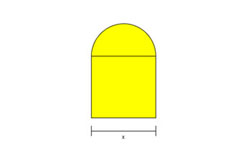
\includegraphics[width=.9\textwidth]{icones-modulos/pot-m-pjn.jpg}
    % \label{fig:pdc-ic}
    \end{subfigure}
    \hfill
    \begin{subfigure}{0.3\textwidth}
    \centering
    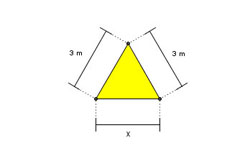
\includegraphics[width=.9\textwidth]{icones-modulos/pot-m-ptr.jpg}
    % \label{fig:pdc-ic}
    \end{subfigure}
    \hfill
    \begin{subfigure}{0.3\textwidth}
    \centering
    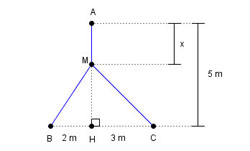
\includegraphics[width=.9\textwidth]{icones-modulos/pot-m-pge.jpg}
    \label{fig:pge-ic}
    \end{subfigure}
    
    \begin{subfigure}{0.3\textwidth}
    \centering
    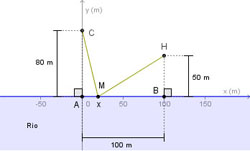
\includegraphics[width=.9\textwidth]{icones-modulos/pot-m-pch.jpg}
    % \label{fig:pch-ic}
    \end{subfigure}
    \hfill
    \begin{subfigure}{0.3\textwidth}
    \centering
    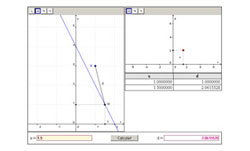
\includegraphics[width=.9\textwidth]{icones-modulos/pot-m-pre.jpg}
    \label{fig:pre-ic}
    \end{subfigure}
    \hfill
    \begin{subfigure}{0.3\textwidth}
    \centering
    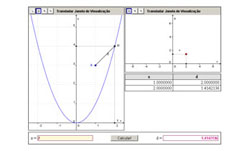
\includegraphics[width=.9\textwidth]{icones-modulos/pot-m-ppa.jpg}
    \label{fig:ppa-ic}
    \end{subfigure}
    
    \begin{subfigure}{0.3\textwidth}
    \centering
    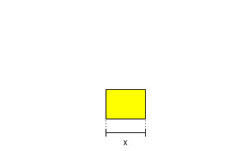
\includegraphics[width=.9\textwidth]{icones-modulos/pot-m-rap.jpg}
    \label{fig:rap-ic}
    \end{subfigure}
    \hfill
    \begin{subfigure}{0.3\textwidth}
    \centering
    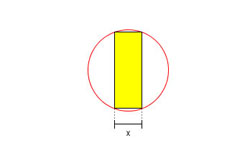
\includegraphics[width=.9\textwidth]{icones-modulos/pot-m-crt.jpg}
    \label{fig:crt-ic}
    \end{subfigure}
    \hfill
    \begin{subfigure}{0.3\textwidth}
    \centering
    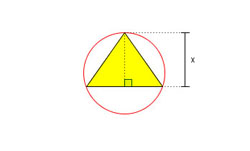
\includegraphics[width=.9\textwidth]{icones-modulos/pot-m-ctr.jpg}
    \label{fig:ctr-ic}
    \end{subfigure}
    
    \begin{subfigure}{0.3\textwidth}
    \centering
    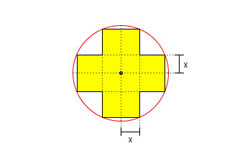
\includegraphics[width=.9\textwidth]{icones-modulos/pot-m-pbo.jpg}
    \label{fig:pbo-ic}
    \end{subfigure}
    \hfill
    \begin{subfigure}{0.3\textwidth}
    \centering
    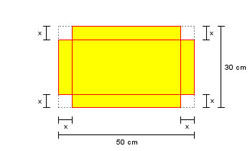
\includegraphics[width=.9\textwidth]{icones-modulos/pot-m-pdc.jpg}
    \label{fig:pdc-ic}
    \end{subfigure}
    \hfill
    \begin{subfigure}{0.3\textwidth}
    \centering
    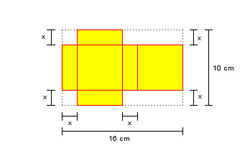
\includegraphics[width=.9\textwidth]{icones-modulos/pot-m-pct.jpg}
    \label{fig:pct-ic}
    \end{subfigure}
    
    
    \begin{subfigure}{0.3\textwidth}
    \centering
    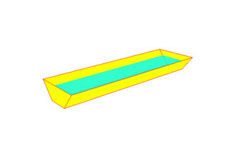
\includegraphics[width=.9\textwidth]{icones-modulos/pot-m-pbe.jpg}
    \label{fig:pbe-ic}
    \end{subfigure}
    \hfill
    \begin{subfigure}{0.3\textwidth}
    \centering
    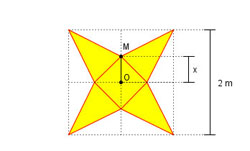
\includegraphics[width=.9\textwidth]{icones-modulos/pot-m-pep.jpg}
    \label{fig:pep-ic}
    \end{subfigure}
    \hfill
    \begin{subfigure}{0.3\textwidth}
    \centering
    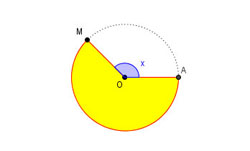
\includegraphics[width=.9\textwidth]{icones-modulos/pot-m-pco.jpg}
    \label{fig:pco-ic}
    \end{subfigure}
    
    \begin{subfigure}{0.3\textwidth}
    \centering
    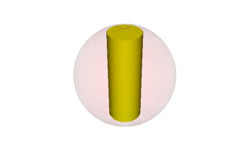
\includegraphics[width=.9\textwidth]{icones-modulos/pot-m-eci.jpg}
    \label{fig:eci-ic}
    \end{subfigure}
    \hfill
    \begin{subfigure}{0.3\textwidth}
    \centering
    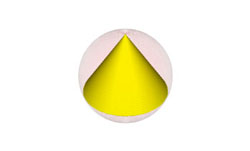
\includegraphics[width=.9\textwidth]{icones-modulos/pot-m-eco.jpg}
    \label{fig:eco-ic}
    \end{subfigure}
    \hfill
    \begin{subfigure}{0.3\textwidth}
    \centering
    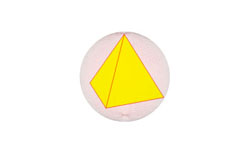
\includegraphics[width=.9\textwidth]{icones-modulos/pot-m-epi.jpg}
    \label{fig:epi-ic}
    \end{subfigure}
    
    \caption{Thumbnails dos módulos do Projeto Ótimo}
    \label{fig:icones-pot}
    
    
\end{figure}